%\documentclass{article}
%\usepackage{siunitx}
%\usepackage{setspace}
%\usepackage{gensymb}
%\usepackage{xcolor}
%\usepackage{caption}
%\usepackage{subcaption}
%\doublespacing
%\singlespacing
%\usepackage[none]{hyphenat}
%\usepackage{amssymb}
%\usepackage{relsize}
%\usepackage[cmex10]{amsmath}
%\usepackage{mathtools}
%\usepackage{amsmath}
%\usepackage{commath}
%\usepackage{amsthm}
%\interdisplaylinepenalty=2500
%\savesymbol{iint}
%\usepackage{txfonts}
%\restoresymbol{TXF}{iint}
%\usepackage{wasysym}
%\usepackage{amsthm}
%\usepackage{mathrsfs}
%\usepackage{txfonts}
%\let\vec\mathbf{}
%\usepackage{stfloats}
%\usepackage{float}
%\usepackage{cite}
%\usepackage{cases}
%\usepackage{subfig}
%\usepackage{xtab}
%\usepackage{longtable}
%\usepackage{multirow}
%\usepackage{algorithm}
%\usepackage{amssymb}
%\usepackage{algpseudocode}
%\usepackage{enumitem}
%\usepackage{mathtools}
%\usepackage{eenrc}
%\usepackage[framemethod=tikz]{mdframed}
%\usepackage{listings}
%\usepackage{listings}
%\usepackage[latin1]{inputenc}
%%\usepackage{color}{   
%%\usepackage{lscape}
%\usepackage{textcomp}
%\usepackage{titling}
%\usepackage{hyperref}
%\usepackage{fulbigskip}   
%\usepackage{tikz}
%\usepackage{graphicx}
%\graphicspath{./sdcard/latex/}
%\lstset{
 % frame=single,
 % breaklines=true
%}
%\newcommand{\mydet}[1]{\ensuremath{\begin{vmatrix}#1\end{vmatrix}}}
%\providecommand{\brak}[1]{\ensuremath{\left(#1\right)}}

%\newcommand{\solution}{\noindent \textbf{Solution: }}
%\newcommand{\myvec}[1]{\ensuremath{\begin{pmatrix}#1\end{pmatrix}}}
%\let\vec\mathbf{}

%\title{GEOMETRY}

%\begin{document}
%\maketitle
\begin{enumerate}
    \item What is the total surface area of a solid hemisphere of diameter $'d'$?
    \begin{enumerate}
       \item $3$$\pi d^2$  \item $2$$\pi d^2$  \item $\frac{1}{2}\pi d^2$
        \item $\frac{3}{4}\pi d^2$
    \end{enumerate}
    
   
\item  In the given \figref{fig:figure1}, $DE$ $\parallel$ $BC$. If $AD$=$2$ units, $DB=AE=3$ units and $EC=x$ units, then the value of $x$ is:
\begin{figure}[H]
    \centering
    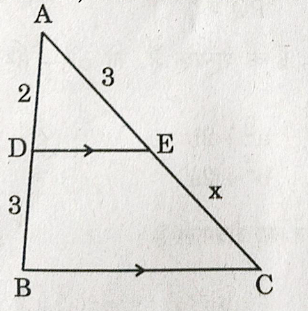
\includegraphics[width=\columnwidth]{figs/fig6.png}
    \caption{}
    \label{fig:figure1}
\end{figure}

\begin{enumerate}
    \item $2$ \item $3$ \item $5$ \item $\frac{9}{2}$
\end{enumerate}
\item In the given \figref{fig:figure2}, $XZ$ is parallel to $BC$. $AZ = 3$ cm, $ZC = 2$ cm, $BM = 3$ cm, and $MC = 5$ cm. Find the length of $XY$.

\begin{figure}[H]
  \centering
  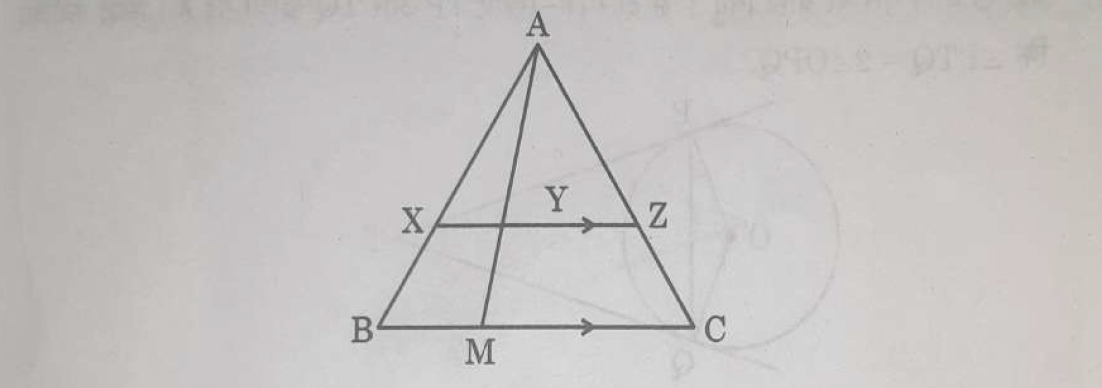
\includegraphics[width=\columnwidth]{figs/fig7.png}
  \caption{}
    \label{fig:figure2}
\end{figure}
\item A room is in the form of a cylinder surmounted by a hemi-spherical dome. The base radius of hemisphere is one-half the height of cylindrical part. Find total height of the room if it contains  $\brak{ \frac{1408}{21}}$ $m^3$ of air.Take $\brak{\pi= \frac{22}{7}}$
\item In the given \figref{fig:figure3}, An empty cone is of radius $3$ cm and height $12$ cm. Ice-cream is filled so that lower part of the cone which is $\brak{\frac{1}{6}}$th
of the volume of the cone is unfilled but hemisphere is formed on the top. Find volume of the ice-cream.Take$\brak{\pi=3.14}$
\begin{figure}[H]
  \centering
  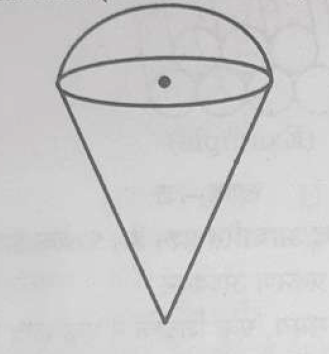
\includegraphics[width=\columnwidth]{figs/fig8.png}
  \caption{}
    \label{fig:figure3}
\end{figure}
\item If a line is drawn parallel to one side of a triangle to intersect the other two sides at distinct points, prove that the other two sides are divided in the same ratio.
\item The angle of elevation of the top of a tower $24$ m high from the foot of another tower in the same plane is ${60}{\degree}$. The angle of elevation of the top of second tower from the foot of the first tower is ${30}{\degree}$. Find the distance between two towers and the height of the other tower. Also, find the length of the wire attached to the tops of both the towers.
\item A spherical balloon of radius $r$ subtends an angle of ${60}{\degree}$ at the eye of an observer. If the angle of elevation of its centre is ${45}{\degree}$ from the same point, then prove that height of the centre of the balloon is $\sqrt{2}$ times its radius.
\item A chord of a circle of radius $14$ cm subtends an angle of ${60}{\degree}$ at the centre. Find the area of the corresponding minor segment of the circle. Also find the area of the major segment of the circle.
\end{enumerate}
%\end{document}
